\documentclass{beamer}
\usetheme{Boadilla}
\usepackage{tikz}
\usepackage{graphicx}
\usepackage{amsmath}
\usetikzlibrary{shapes.geometric,arrows, positioning, fit}
\tikzstyle{computing} = [draw, rectangle, fill=white!50, rounded corners, node distance=2cm,
                    minimum height=3em]

\tikzstyle{io} = [rectangle, draw, trapezium right angle=110, rounded corners,
                  fill=red!20, node distance=1.9cm, minimum height=2.9em]

\tikzstyle{calculate} = [diamond, draw, trapezium right angle=110, rounded corners,
                  fill=green!20, node distance=1.9cm, minimum height=2.9em]

\tikzstyle{hardware} = [rectangle, draw, trapezium right angle=110, rounded corners,
                  fill=blue!20, node distance=1.9cm, minimum height=2.9em]

\tikzstyle{external} = [rectangle, draw, trapezium right angle=110, rounded corners,
                  fill=gray!20, node distance=1.9cm, minimum height=2.9em]
\tikzstyle{line} = [draw, -latex']

\tikzstyle{function} = [rectangle, draw, fill=green!20, node distance=1.9cm, minimum height=2.9em]
\tikzstyle{ros} = [circle, draw,
                  fill=gray!20, node distance=1.9cm, minimum height=2.9em]

                  \tikzstyle{Process} = [rectangle, draw]

                  \tikzstyle{Start} = [draw, rectangle, rounded corners] 
                  
                  \tikzstyle{Data} = [draw,trapezium,trapezium left angle=70,trapezium right angle=-70]





\title{Weekly Presentation}
\subtitle{Week 43}
\author{}
\institute{Luleå University of Technology}
\date{\today}



\begin{document}
\begin{frame}
    \titlepage
\end{frame}

\begin{frame}
    \frametitle{Overview}
    \tableofcontents
\end{frame}


%%%%%%%%%%%% Add new frames below this line %%%%%%%%%
\section{Project structure}
\begin{frame}
    \subsection{Team}
    \frametitle{Group members }
    \begin{itemize}
        \item Y-students
        \begin{itemize}
            \item Martin Blaszczyk - Project leader and object detection
            \item Edward Cedergård -Arm and gripping tool
            \item Niklad Dahlqvist -  Arm and gripping tool
            \item Måns Norell - Movable base
        \end{itemize}
        \item D-students
        \begin{itemize}
            \item Edward Källstedt - Object detection
            \item Albin Martinsson - Arrowhead and Git
        \end{itemize}  
    \end{itemize}
\end{frame}
\begin{frame}
    \subsection{Time plan}
    \frametitle{Overall timetable}
    \begin{table}
        \begin{tabular}{| l | c | c | c | c }
            
            Sep & Oct & Nov & Dec \\
            \hline \hline
            Concept generation & Evaluation & Evaluation &  \\ 
            \hline
            Theory & Prototyping & Evaluation & Finishing up \\
            \hline
            Simulation & Evaluation & Evaluation & \\
            \hline
            Prototyping & Final Design & Evaluation &  \\
            \hline
 
        \end{tabular}
    \end{table}    
\end{frame}

\begin{frame}
    
    \frametitle{Time plan for October}
    \begin{table}
        \begin{tabular}{l | c | c | c | c }
        Subproject & Week 1 & Week 2 & Week 3 & Week 4 \\
        \hline \hline
            Arrow & Working & Structure & Fusion & ...\\
            Base & CAD & Communication & ROS & Final\\
            Arm  & Assembly & Gripper & ROS & Final\\
            MV & Porting to NVIDIA & API & Evaluation & ...\\
        \end{tabular}
    \end{table}
\end{frame}



\section{Engineering challenge}
\section*{Mechanical structure}
The final design of the robot. Include CAD renderings etc. 
\section*{Electrical components}
Electrical components such as motors, MCUs etc. Why were they chosen




\begin{frame}
    \frametitle{NVIDIA Jetson Nano}
    \begin{columns}
        \begin{column}[]{0.5\textwidth}
            \begin{itemize}
                \item Runs Ubuntu
                \item Two camera ports (CSI)
                \item More powerful GPU than RPi
            \end{itemize}
        \end{column}

        \begin{column}[]{0.5\textwidth}
            \includegraphics[width=\textwidth]{frames/img/nvidia.jpg}
        \end{column}
    \end{columns}


\end{frame}

\begin{frame}
    \frametitle{Cameras}
    \begin{columns}
        \begin{column}[]{0.5\textwidth}
            \begin{itemize}
                \item Compatible with NVIDIA and RPi
                \item Small package
                \item 8 megapixels
                \item Video:
                \begin{itemize}
                    \item 1080p @ 30 fps
                    \item 720p @ 60fps
                \end{itemize}

            \end{itemize}
        \end{column}

        \begin{column}[]{0.5\textwidth}
            \includegraphics[width=\textwidth]{frames/img/camera.jpg}
        \end{column}
    \end{columns}
\end{frame}


\begin{frame}
    \frametitle{Dynamixel Smart Motors}
    \begin{columns}
        \begin{column}[]{0.5\textwidth}
            \begin{itemize}
                \item Connects in series
                \item Angle and wheel mode
                \item Feedback
            \end{itemize}
        \end{column}

        \begin{column}[]{0.5\textwidth}
            \includegraphics[width=\textwidth]{frames/img/dynamixel.png}
        \end{column}
    \end{columns}
\end{frame}

\begin{frame}
    \frametitle{Hardware}
    \centering
    \resizebox{7.0cm}{!}{
    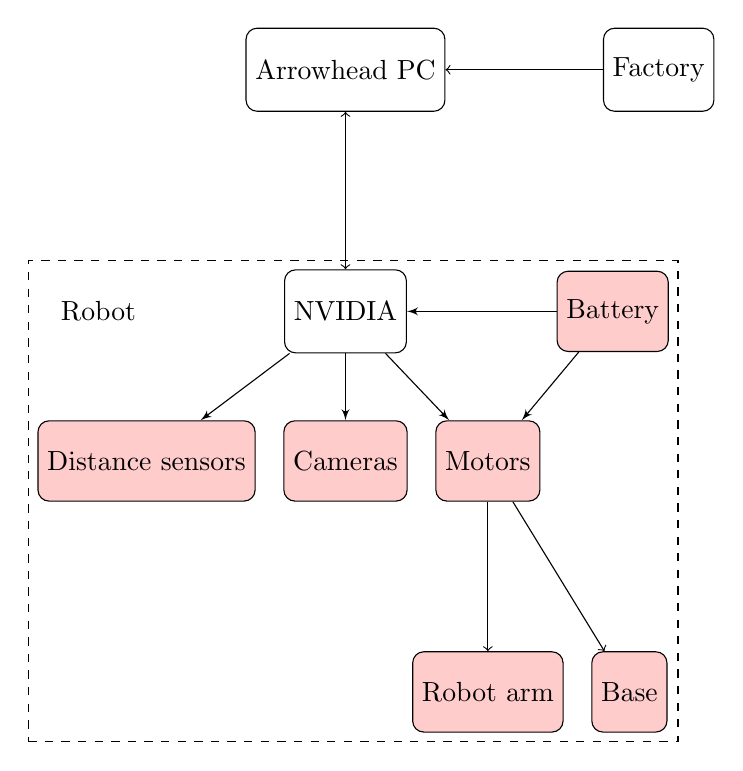
\begin{tikzpicture}
        [align=center, node distance=1em, auto]

        \node [computing] (pc) {Arrowhead PC};
        \node [computing, below= of pc] (nvidia) {NVIDIA};
        \node [io, right= of nvidia] (battery) {Battery};
        \node [computing, right= of pc] (factory) {Factory};
        \node [io, below of= nvidia] (cameras) {Cameras};
        \node [io, right= 1em of cameras] (motors) {Motors};
        \node [io, left= 1em of cameras] (distance_sensors) {Distance sensors};
        \node [io, below= of motors] (arm) {Robot arm};
        \node [io, right= 1em of arm] (base) {Base};
        \node [rectangle=white, left= 5em of nvidia] (robot) {Robot};

        \path [line] (nvidia)--(cameras);
        \path [line] (battery)--(nvidia);
        \path [line] (battery)--(motors);
        \path [line] (nvidia)--(motors);
        \path [line] (nvidia)--(distance_sensors);
        \draw[->] (factory) -- (pc);
        \draw[<->] (pc) -- (nvidia);
        \draw[->] (motors) -- (arm);
        \draw[->] (motors) -- (base);
        \node [draw=black, dashed, fit= (nvidia) (battery) (distance_sensors)
        (cameras) (motors) (base) (arm)]{};

    \end{tikzpicture}
    }
\end{frame}


\begin{frame}
    \frametitle{Concept rendering}
    \includegraphics[width=\textwidth]{frames/img/b4_manufacturing.PNG}
\end{frame}
\begin{frame}
\frametitle{Positioning - Arrowhead}

\begin{center}
    

\resizebox{9.0cm}{!}{

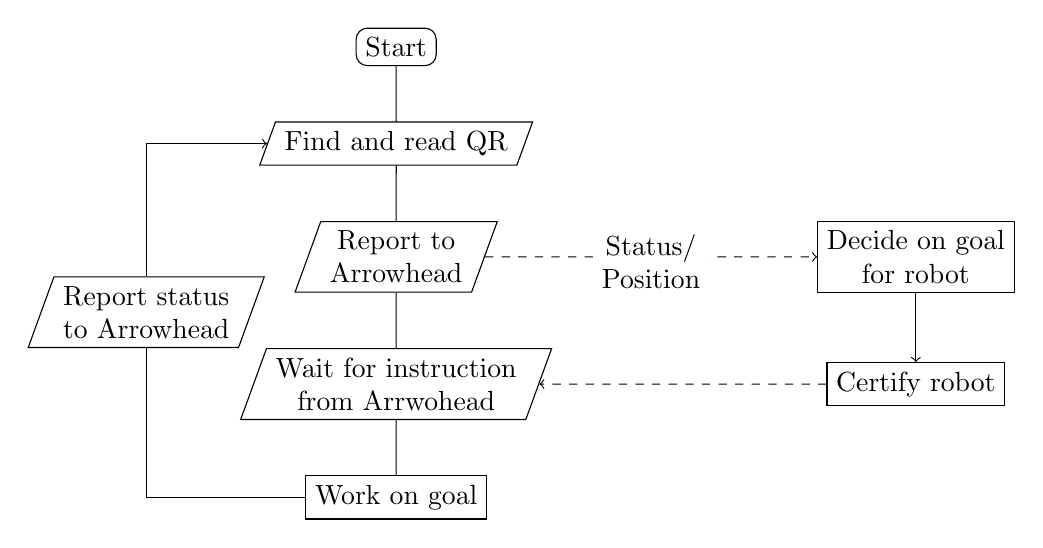
\begin{tikzpicture}
    [align=center, node distance = 2em,  auto]

    %% Robot
    \node [Start] (start) {Start};
    \node [Data, below= of start] (findqr) {Find and read QR};
    \node [Data, below= of findqr] (report) {Report to \\ Arrowhead};
    \node [Data, below= of report] (getgood) {Wait for instruction \\from Arrwohead};
    \node [Process, below= of getgood] (follow) {Work on goal};
    \node [Data, left= of report, yshift=-2em] (status) {Report status \\ to Arrowhead};

    %% Arrowhead
    \node [Process, right= of report, xshift=10em] (arrowstart) {Decide on goal \\ for robot};
    \node [Process, below= of arrowstart, yshift=-0.5em] (certify) {Certify robot};


    %% Draw
    \draw (start) -- (findqr) -- (report) -- (getgood) -- (follow);
    \draw [->] (follow) -| (status) |- (findqr);

    
    \draw [->, dashed] (report) -- node[midway, fill=white, yshift=-1.5em] {Status/ \\ Position} (arrowstart);
    \draw [->] (arrowstart) -- (certify);
    \draw [->, dashed] (certify) -- (getgood);

\end{tikzpicture}
}
\end{center}
\end{frame}
\begin{frame}
    \frametitle{ROS-Base example}
\begin{center}
    

    \resizebox{8.0cm}{!}{
    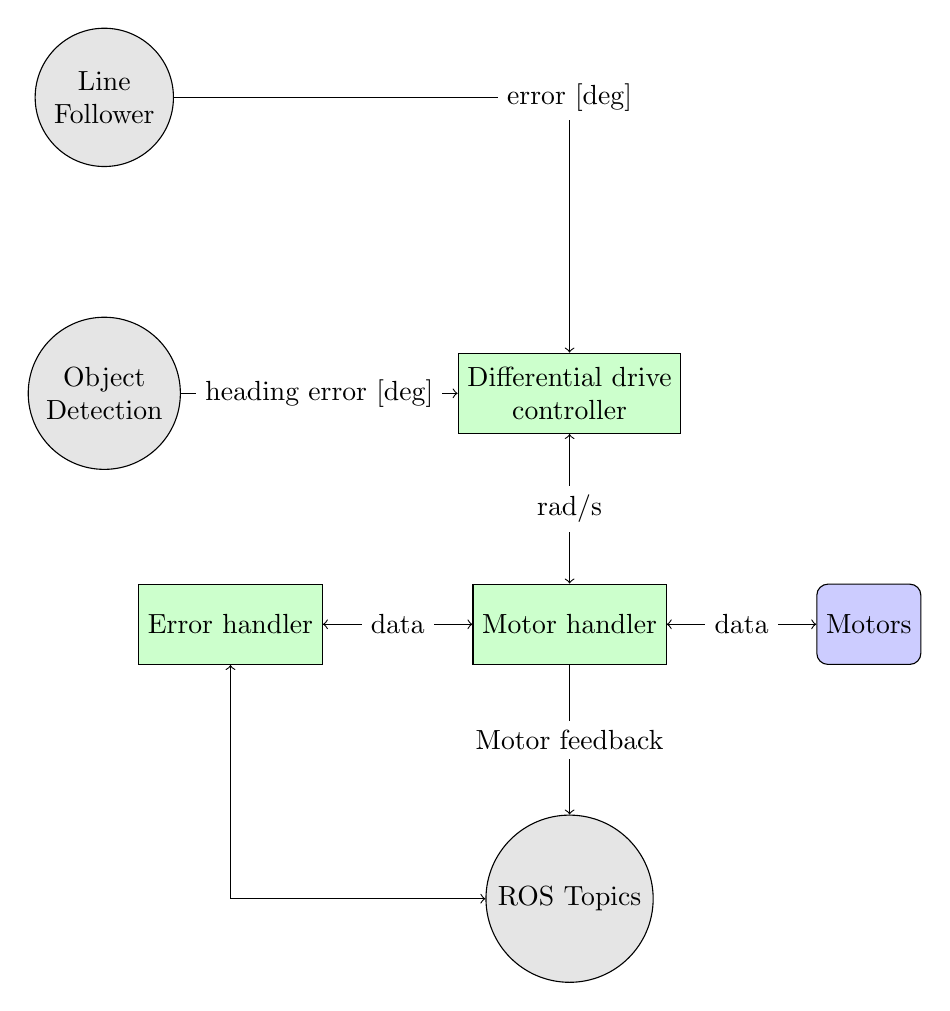
\begin{tikzpicture}
        [align=center]
        \node [ros] (line) {Line \\Follower};
        \coordinate [below= of line] (aux1);
        \node [ros, below= of line] (obj) {Object\\ Detection};
        \node [function, right= 10em of obj] (diff) {Differential drive\\controller};
        \node [function, below= of diff] (handler) {Motor handler};
        \node [function, left= of handler] (error) {Error handler};
        \node [hardware, right= of handler] (motors) {Motors};
        \node [ros, below= of handler] (ros) {ROS Topics};
    
        
        
    
        \draw [->] (line) -| node[midway, fill=white] {error [deg]} (diff);
        \draw [<->] (diff) -- node[midway, fill=white] {rad/s} (handler);
        \draw [<->] (handler) -- node[midway, fill=white] {data} (motors);
        \draw [->] (handler) -- node[midway, fill=white] {Motor feedback} (ros);
        \draw [->] (obj) -- node[midway, fill=white] {heading error [deg]} (diff);
        \draw [<->] (error) -- node[midway, fill=white] {data} (handler);
        \draw [<->] (error) |- (ros);
        
    \end{tikzpicture}
    }
\end{center}
\end{frame}
\input{frames/factory.tex}





%%%%%%%%%%%% Add new frames above this line %%%%%%%%%


\begin{frame}
    \begin{center}
        \Huge Questions?
    \end{center}
\end{frame}





\end{document}